\documentclass{hw}
\usepackage{mhchem}
\usepackage{nuc}
\usepackage[load=addn]{siunitx}
\usepackage{amsmath}
\usepackage{cancel}
\usepackage{physics}
\graphicspath{ {images/}}

\author{J.R. Powers-Luhn}
\date{2016/11/22}
\title{Homework No. 6}

\begin{document}


\section{}
The NESTLE simulator was run with the provided input. The runtime was approximately 20 minutes, though that varied based on load on the specific cluster node employed. It was also possible to run the simulator on the virtual machine provided, without real performance degradation, but recovering the output files proved more challenging than expected.

\section{}
The output from the NESTLE simulator first describes the configuration with which the simulator was run. It appears to describe a system with two delayed neutron groups, two neutron energy groups, two values for buckling\footnote{It is not specified whether this refers to material or geometric buckling. Since there are two neutron groups, it could be either. In any case, each has the same value, \num{0.67e-4}}, and scattering\footnote{Scattering values for each group to the other group are \num{0}}. Neutron velocities for each group are given as \SI{1.25e7}{\centi\meter\per\second} and \SI{2.5e5}{\centi\meter\per\second}. Each of these values is given in terms of fuel burnup, and the scattering cross sections change as burnup increases (seen in line 2296 of the output file). Coolant density corrections due to temperature are also applied, allowing for variations in the scattering cross sections in the core. As burnup increases, the simulator tracks absorption cross sections for two fission product poisons of concern, \ce{Xe} and \ce{Sm}. The simulator also tracks the contribution of decay heat to overal reactor output.

\section{}
\begin{figure}
    \centering
    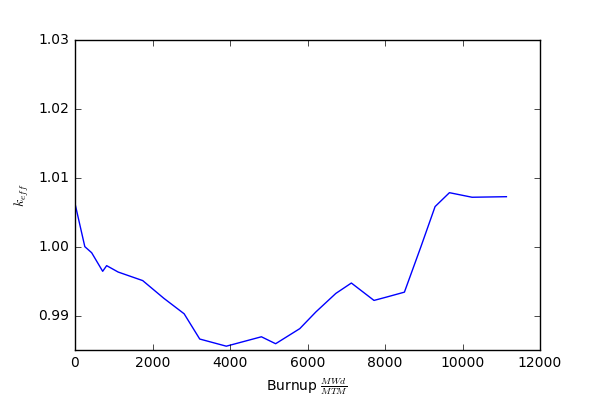
\includegraphics[width=0.5\textwidth]{k_eff_normal}
    \caption{$k_{eff}$ vs fuel burnup}    
    \label{fig:k_eff_normal}
\end{figure}
A plot of $k_{eff}$ vs burnup was prepared and can be seen in figure \ref{fig:k_eff_normal}. As the core continues to operate, a variety of factors influence the effective multiplication factor including coolant temperature, rod height, and poison buildup. This means that the core, even while sustaining at-power operations, will see variations in reactivity/$k_{eff}$ as fluctuations in the core occur and are compensated for by the control systems.

\section{}
The input file was modified to simulate a core with all rods out and a constant power production with constant input (cold leg) and output (hot leg) coolant temperatures. This was matched with a constant 100\% power and flow setting for the duration of core operations. Finally, burnup values were extended out to \SI{20000}{\mega\watt\day\per\mega\tonne}. A plot of $k_{eff}$ vs burnup for this core is shown in figure \ref{fig:k_eff_aro}.

\begin{figure}
    \centering
    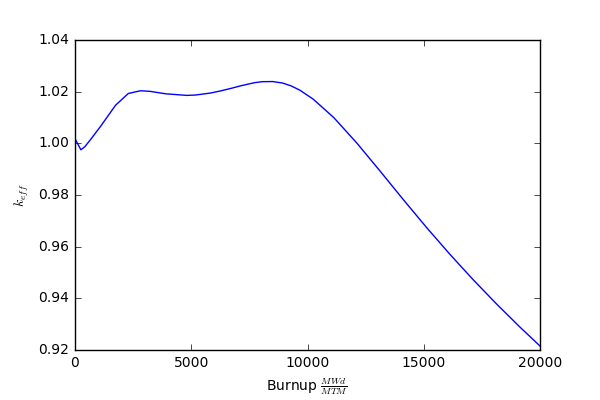
\includegraphics[width=0.9\textwidth]{k_eff_aro}
    \caption{$k_{eff}$ vs fuel burnup, all rods out}
    \label{fig:k_eff_aro}
\end{figure}

Since this second round of simulation controls for all reactivity sources except fuel and fission product poisons (control rod insertion, moderator temperature/density, etc), it is trivial to produce a graph of excess reactivity as a function of fuel burnup--and this graph can be seen in \ref{fig:reactivity_aro}. This shows an initial drop in excess reactivity as fission product poisons start to build up and are burned off, eventually reaching equilibrium values as the poison precursors decay, followed by the fuel consumption dominating as $N_{fuel} \downarrow \rightarrow \Sigma_f \downarrow$. Finally, even with all rods out, there is not enough reactivity to sustain critical operations at temperature. This occurs sometime around \SI{12000}{\mega\watt\day\per\mega\tonne}.

\begin{figure}
    \centering
    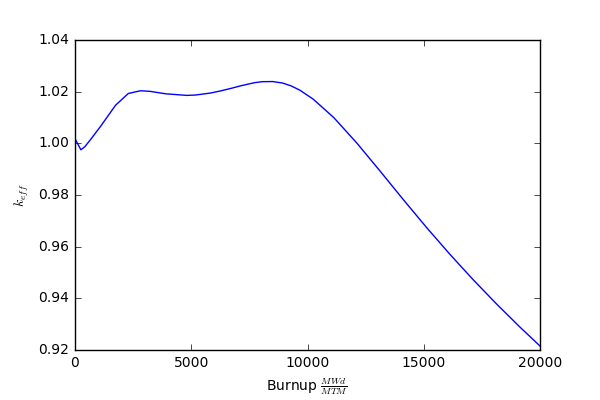
\includegraphics[width=0.9\textwidth]{k_eff_aro}
    \caption{$\rho_{excess}$ vs fuel burnup, all rods out}
    \label{fig:reactivity_aro}
\end{figure}

\end{document}